\documentclass[11pt,a4paper,french,twoside]{PMCours}
\usepackage{hyperref}
\usetikzlibrary{chains,fit,shapes}

\newcounter{activite}
\newcommand{\activite}{\subsubsection*{Activité~\refstepcounter{activite}\theactivite}}

\begin{document}
\TitreISN{Classe de Terminale}{Année 2021--2022}
{Numérique et Sciences Informatiques}{TP : Machine de Turing.}


%\tableofcontents

%\newpage

\section{Introduction}

\subsection{Calculabilité}
En informatique théorique, une question importante est de savoir ce qu'il est 
possible ou non de calculer en utilisant des algorithmes. C'est ce qu'on appelle
la calculabilité.

\medskip
Pour pouvoir aborder cette que question, il est nécessaire de définir précisément
ce qu'est un algorithmes et comment on l'exécute. On a donc besoin de modèle
abstrait permettant l'exécution de programmes.

\medskip
La machine de Turing a été proposée par Alan Turing en 1936. Elle fournit l'une
des deux principales approchent de la calculabilité, l'autre étant le 
$\lambda$-calcul.

\medskip
Il s'agit de deux approches franchement différentes, et pourtant, elles
donnent des résultats complètement équivalents sur la calculabilité. 
Il se pourrait donc que la calculabilité soit quelque chose de plus profond.
Mais cela est une histoire qui nous intéressera plus tard.

\medskip
L'objectif de ce TP est de programmer une machine de Turing, afin de se 
familiariser avec son fonctionnement. Ce qui nous permettra de parler de 
calculabilité avec plus de facilité.


\subsection{La machine de Turing}
La machine de Turing est constitué ainsi :
\begin{itemize}
  \item Un ruban de mémoire infini, dans les deux directions, portant les 
  symboles d'un alphabet. Le ruban portera pour nous des 0, des 1 et des $\bullet$
  qui représente un blanc.
  \item Une tête de lecture/écriture pouvant se déplacer d'un cran vers la droite
  ou la gauche ou restant sur place.
  \item Un état pris dans une liste finie.
  \item Une table de règles de transition qui représente le programme. Les règles
  disent, pour un état de la machine et le symbole se trouvant sur le ruban à 
  l'emplacement de la tête, ce qu'il faut écrire, dans quel direction déplacer 
  la tête et le nouvel état de la machine.
\end{itemize}

\medskip
Voici un schéma de la machine. On remarque son ruban infini, la tête de 
lecture/écriture, $q_1$ est l'état actuel de la machine.  
\begin{center}
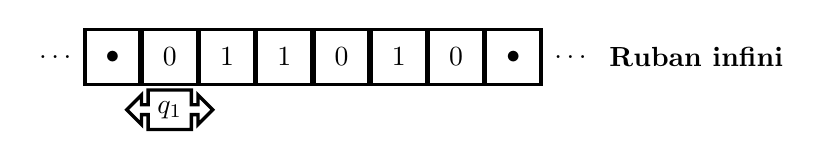
\begin{tikzpicture}
\tikzstyle{every path}=[very thick]

\edef\sizetape{0.7cm}
\tikzstyle{tmtape}=[draw,minimum size=\sizetape]
\tikzstyle{tmhead}=[arrow box,draw,minimum size=.5cm,arrow box
arrows={east:.25cm, west:0.25cm}]

%% Draw TM tape
\begin{scope}[start chain=1 going right,node distance=-0.15mm]
    \node [on chain=1,tmtape,draw=none] {$\ldots$};
    \node [on chain=1,tmtape] {$\bullet$};
    \node [on chain=1,tmtape] (input) {0};
    \node [on chain=1,tmtape] {1};
    \node [on chain=1,tmtape] {1};
    \node [on chain=1,tmtape] {0};
    \node [on chain=1,tmtape] {1};
    \node [on chain=1,tmtape] {0};
    \node [on chain=1,tmtape] {$\bullet$};
    \node [on chain=1,tmtape,draw=none] {$\ldots$};
    \node [on chain=1] {\textbf{Ruban infini}};
\end{scope}

%% Draw TM head below (input) tape cell
\node [tmhead,yshift=-.3cm] at (input.south) (head) {$q_1$};
\end{tikzpicture}
\end{center}

\medskip


\section{Implémentation}
\subsection{Le ruban}
\subsection{La machine de Turing}


\subsection{Exercices}


\end{document}
